\chapter{Modelo Preditivo de Controle}
\label{ch:mpc}

% TODO: Utilizar
% \cite{Haugen2018}
% O \acrshort{mpc} tem como princípio calcular a melhor sequência de variáveis de controle sob um dado
% futuro ou horizonte de tempo baseando-se no modelo do processo, valores dos estados atuais (medidos e estimados),
% valores de \textit{setpoint}, distúrbios conhecidos e limitantes das variáveis de controle, variáveis de
% processo e variáveis de estado.

% \cite{Haugen2018}
% o MPC produz o sinal de controle que fornece o melhor equilíbrio entre erros de controle e mudanças
% de sinal de controle. Não é possível obter erros de controle muito pequenos e alterações de sinal de
% controle muito pequenas. Portanto, um equilíbrio sempre existirá.

Segundo \citeonline{Rossiter2003} uma das principais diferenças entre o \acrshort{mpc} e a maioria das
leis de controle (como o \acrshort{pid}, por exemplo) é que a maioria delas não leva em consideração
as ações futuras do controle, porém o \acrshort{mpc} sim, e para essas ações futuras sejam consideradas
é necessário possuir um modelo do sistema que mostre as dependências das saídas e das atuais variáveis
medidas e as entradas atuais e futuras. % TODO: Conferir traducao deste pedaco. Rossiter pag 2
Este modelo não precisa ser linear, e nem tão pouco ser extremamente fiel em descrever todas as interações
físico-químicas do sistema. Na verdade, a regra básica do modelo, ainda segundo \citeonline{Rossiter2003}
é que ele deve ser o mais simples possível, ou seja, deve ser o modelamento mínimo necessário para que
possamos observar predições com o nível de precisão necessário.

Além de comparar com outros métodos de controle e de descrever os modelos utilizados no \acrshort{mpc},
\citeonline{Rossiter2003} também salienta alguns parametros e características que são importantes importantes
para a técnica. Eles são descritos nos itens a seguir:

\begin{itemize}
    \item \textbf{Selecionar as entradas}
        % TODO: Teminar daqui
    
\end{itemize}


% =====================================================================================================
% ============================================= Section ===============================================
% =====================================================================================================
\section{Aplicação prática}
\label{sec:aplicacao_pratica}

Segundo \citeonline{Haugen2018} tanto o \acrshort{mpc} quanto o \acrshort{mhe} são problemas praticamente
identicos do ponto de vista matemático, pois ambos exploram um modelo matemático sobre dado um horizonte de
tempo, porém, apesar de matematicamente parecidos, eles atuam de forma inversa um ao outro, pois
enquanto o \acrshort{mhe} utiliza as variáveis de controle e os valores medidos do processo para estimar
as variáveis estados (como já apresentado na \cref{subsec:moving_horizon_estimation}), o \acrshort{mpc}
utiliza as variáveis de estado e os valores medidos do processo para estimar as variáveis de controle.
Na \cref{fig:mhe_mpc} é possível observar o \acrshort{mhe} atuando sob um horizonte de estimação, utilizando
dados passados, e o \acrshort{mpc} atuando dob um horizonte de predição, predizendo os valores futuros.

\begin{figure}
	\begin{center}
		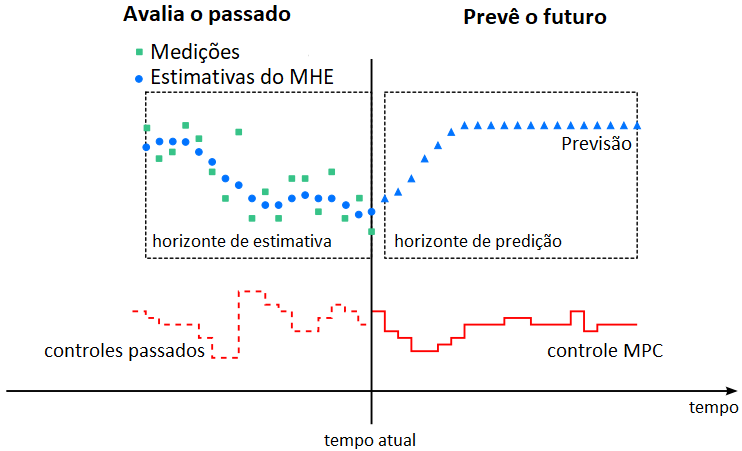
\includegraphics[width=0.9\textwidth]{./5_images/fig_mhe_mpc.png} 
		\caption{Ação do \acrlong{mhe} e do \acrlong{mpc}}
		\label{fig:mhe_mpc}
		\makebox[\width]{Fonte: \citeonline{Vukov2015a}}
	\end{center}
\end{figure}

Podemos descrever o \acrshort{mpc} através de um problema de otimização de forma análoga ao que foi feito
na \cref{subsec:moving_horizon_estimation} para descrever o \acrshort{mhe}, porém, ao invés minimizarmos
as variáveis de estado, devemos encontrar os valores ótimos (minimizar) das variáveis de controle.
As \crefrange{eq:mpc_minimization}{eq:mpc_minimization3} descrevem este problema de otimização.

\begin{equation}
	\label{eq:mpc_minimization}
	\min_{U} \sum_{i=k}^{k+N} ( \Vert e_i \Vert^2_{C_e} + \Vert du \Vert^2_{C_{du}} )
\end{equation}

\noindent
Onde: 
\begin{itemize}
	\item $\mathrm{U}$ é uma matriz contendo $r$ variáveis de controle nos instantes $k$ do horizonte de predição.
        \begin{equation}
            \label{eq:mpc_control_signal_matrix}
            \begin{aligned}
                \mathrm{U} &= [\mathrm{u}_{k}, \mathrm{u}_{k+1}, \cdots, \mathrm{u}_{k+(N-1)}, \mathrm{u}_N] \\
                &=
                \begin{bmatrix}
                    u(1)_{k} & u(1)_{k+1} & \cdots & u(1)_{k+(N-1)} & u(1)_N		\\
                    u(2)_{k} & u(2)_{k+1} & \cdots & u(2)_{k+(N-1)} & u(2)_N		\\
                    \vdots & \vdots & \ddots & \vdots & \vdots						\\
                    u(n)_{k} & u(n)_{k+1} & \cdots & u(n)_{k+(N-1)} & u(n)_N	
                \end{bmatrix}
            \end{aligned}
        \end{equation}
		
	\item $\mathrm{e}_i$ é o vetor de erro de controle
		\begin{equation}
			\mathrm{e}_i =
			\begin{bmatrix}
				e(1)_i \\
				e(2)_i \\
				\vdots \\
				e(m)_i \\
			\end{bmatrix}
        \end{equation}
        
        Onde $e(j)_i$ é o erro de controle da saída $j$ do processo, no instante de tempo $i$, sendo que:

        \begin{equation}
			e(j)_i = y(j)_{sp_i} - y(j)_i               % TODO: Explicar o que é cada termo?
        \end{equation}
		
	\item $\mathrm{du}_i$ é o vetor de incremento da variável de controle
        \begin{equation}
            \mathrm{du}_i =
            \begin{bmatrix}
                du(1)_i \\
                du(2)_i \\
                \vdots \\
                du(r)_i \\
            \end{bmatrix}
        \end{equation}

        Onde $du(j)_i$ é o incremento da variável de controle relativo à esta mesma variável no instante
        de tempo anterior:

        \begin{equation}
			du(j)_i = u(j)_i - u(j)_{i-1}
        \end{equation}
	
	\item As matrizes $\mathrm{C_e}$ e $\mathrm{C_{du}}$ são matrizes de custo (peso) e são utilizadas
        como elementos de sintonia.

        \begin{subequations}
            \label{eq:mpc_cost_matrix}
            \begin{align}
                \mathrm{C_e} &= 
                \begin{bmatrix}
                    C_e(1,1) & \cdots & 0   		\\
                    \vdots & \ddots & \vdots		\\
                    0 & \cdots & C_e(m,m)	
                \end{bmatrix}
                                                    \\
                \mathrm{C_{du}} &= 
                \begin{bmatrix}
                    C_{du}(1,1) & \cdots & 0   		\\
                    \vdots & \ddots & \vdots		\\
                    0 & \cdots & C_{du}(r,r)	
                \end{bmatrix}
            \end{align}
        \end{subequations}
	
\end{itemize}

Substituindo as normas matriciais da \cref{eq:mpc_minimization}, temos:

\begin{equation}
    \label{eq:mpc_minimization2}
    \min_{U} \sum_{i=k}^{k+N} ( e^T_i C_e e_i + du^T_i C_{du} du_i )
\end{equation}

Expandindo então as \crefrange{eq:mpc_control_signal_matrix}{eq:mpc_cost_matrix} na \cref{eq:mpc_minimization2},
obtemos:

\begin{equation}
    \label{eq:mpc_minimization3}
    \min_{U} \sum_{i=k}^{k+N} [C_e(1,1) e(1)^2_i + \cdots + C_e(m,m) e(m)^2_i] + 
                                [C_{du}(1,1) du(1)^2_i + \cdots + C_{du}(r,r) du(r)^2_i]
\end{equation}

% TODO: Incluir itens da pág 90? Constrains, Guessed value of U, etc???

% .....................................................................................................
% ............................................ Subsection .............................................
% .....................................................................................................
\subsection{Exemplo}
\label{subsec:mpc_example}

O exemplo descrito nesta seção apresenta a simulação do modelo de uma planta didática de aquecimento de ar
utilizado na University College of Southeast Norway, situada em Porsgrunn, Noruega. O modelo matemático
desta planta é descrito na \cref{eq:heat_plant} abaixo.

\begin{subequations}
    \label{eq:heat_plant}
    \begin{align}
        {\theta}_t \dot{T}_{heat} (t) &= -T_{heat} (t) + K_h [u(t - {\theta}_d) + d]     \\
        T_{out} (t) &= T_{heat} (t) + T_{env}
    \end{align}
\end{subequations}

\noindent
Onde: 
\begin{itemize}
	\item $K_h$ é o ganho do aquecedor
	\item $T_{env}$ é a temperatura ambiente
	\item $T_{heat}$ é a contribuição para a temperatura total $T_{out}$ devido ao aquecedor
	\item $T_{out}$ é a temperatura do ar saindo da planta. Medido através de sensor
	\item $u$ é o sinal de controle do aquecedor
	\item $d$ é o distúrbio de entrada (adicionado ao sinal de controle)
	\item ${\theta}_d$ é o atraso que representa o transporte de ar e a dinâmica do aquecedor
	\item ${\theta}_t$ é o atraso referente a dinâmica do aquecedor
\end{itemize}

A \cref{fig:mpc_example} ilustra os dados obtidos através da execução do código-fonte \ref{lst:mpc_example}
escrito em Python.

\begin{figure}[h]
	\begin{center}
		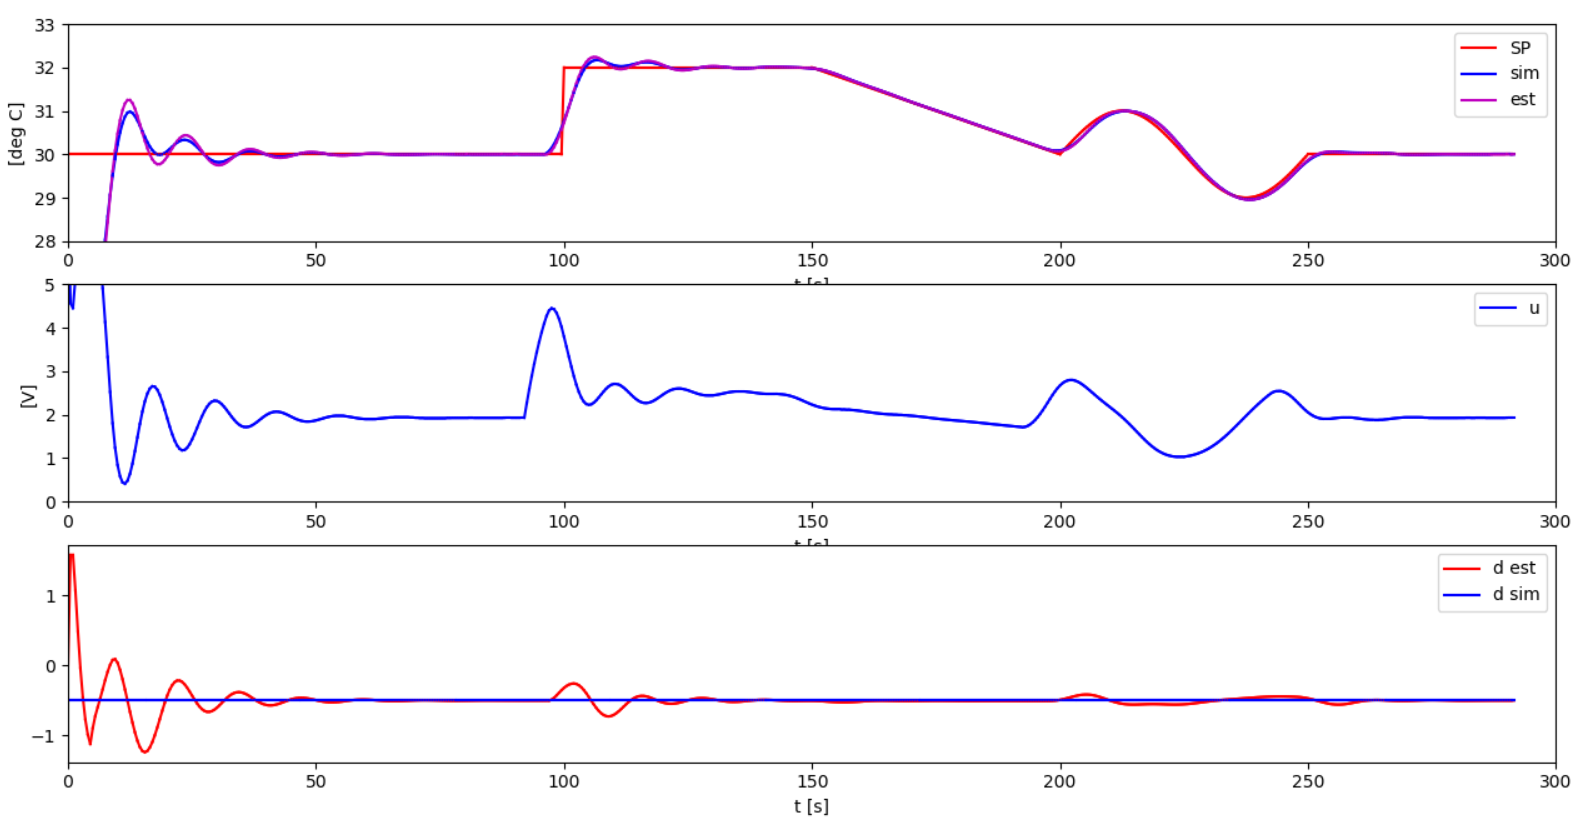
\includegraphics[width=1\textwidth]{./5_images/fig_mpc_example.png} 
		\caption{Simulação utilizando \acrlong{mpc}}
		\label{fig:mpc_example}
		\makebox[\width]{Fonte: Autor, adaptado de \citeonline{Haugen2018}}
	\end{center}
\end{figure}

\lstinputlisting[	
	caption={[Exemplo de aplicação do \acrlong{mpc}]
	Exemplo de aplicação do \acrlong{mpc} \\
	Fonte: Autor, adaptado de \citeonline{Haugen2018}},
	label={lst:mpc_example},
	language=Python,
	style=Python_lang]
	{./4_Codes/mpc_example.py}

% =====================================================================================================
% ============================================= Section ===============================================
% =====================================================================================================
\section{Algoritmos}
\label{sec:algoritmos}

% TODO: algo

% .....................................................................................................
% ............................................ Subsection .............................................
% .....................................................................................................
\subsection{LQG}
\label{subsec:lqg}

% TODO: LQG

% .....................................................................................................
% ............................................ Subsection .............................................
% .....................................................................................................
\subsection{IDCOM}
\label{subsec:idcom}

% TODO: IDCOM

% .....................................................................................................
% ............................................ Subsection .............................................
% .....................................................................................................
\subsection{DMC}
\label{subsec:dmc}

% TODO: DMC

% .....................................................................................................
% ............................................ Subsection .............................................
% .....................................................................................................
\subsection{QDMC}
\label{subsec:qdmc}

% TODO: QDMC

% .....................................................................................................
% ............................................ Subsection .............................................
% .....................................................................................................
\subsection{IDCOM-M, HIECON, SMCA e SMOC}
\label{subsec:idcomm}

% TODO: IDCOM-M

% .....................................................................................................
% ............................................ Subsection .............................................
% .....................................................................................................
\subsection{DMC-plus e RMPCT In}
\label{subsec:dmcplus}

% TODO: DMC-plus